\chapter{Testing Programs}
\label{chap:testing}
A software bug is an error in a computer program that causes it to produce an incorrect result or behave in an unintended manner. The term 'bug' was used by Thomas Edison in 1878\footnote{\url{https://en.wikipedia.org/wiki/Software_bug}}\footnote{\url{http://edison.rutgers.edu/NamesSearch/DocImage.php3?DocId=LB003487}}, but made popular in computer science by Grace Hopper, who found a moth interfering with the electronic circuits of the Harward Mark II electromechanical computer and coined the term \idx{bug} for errors in computer programs. The original bug is shown in \Cref{fig:bug}.
\begin{figure}
  \centering
  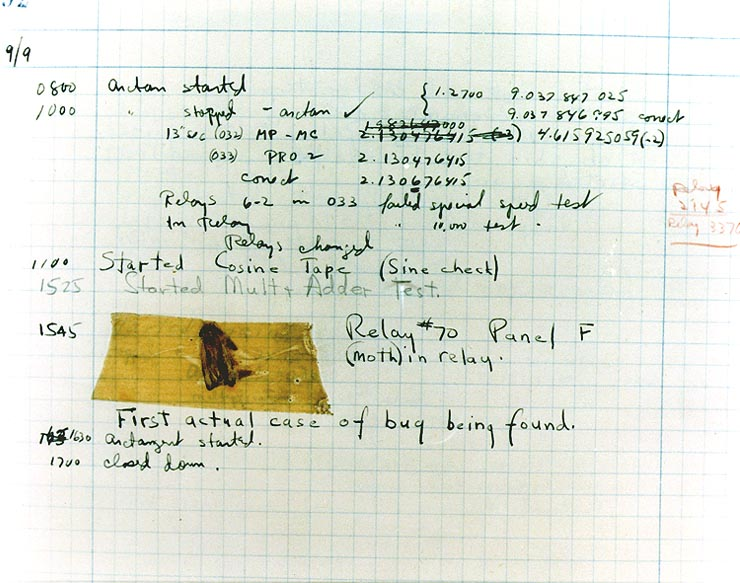
\includegraphics[width=0.45\linewidth]{H96566k}
  \caption{The first computer bug, caught by Grace Hopper, U.S. Naval Historical Center Online Library Photograph NH 96566-KN.}
  \label{fig:bug}
\end{figure}
Software is everywhere, and errors therein have a huge economic impact on our society and can threaten lives\footnote{\url{https://en.wikipedia.org/wiki/List_of_software_bugs}}.

The ISO/IEC organizations have developed standards for software testing\footnote{ISO/IEC 9126, International standard for the evaluation of software quality, December 19, 1991, later replaced by ISO/IEC 25010:2011}.  To illustrate basic concepts of software quality, consider a hypothetical route planning system. Essential factors of its quality are:
\begin{description}
\item[Functionality:]\idxs{functionality} Does the software compile and run without internal errors. Does it solve the problem it was intended to solve? E.g., does the route planning software find a suitable route from point a to b?
\item[Reliability:]\idxs{reliability} Does the software work reliably over time? E.g., does the route planning software work when there are internet dropouts?
\item[Usability:]\idxs{usability} Is the software easy and intuitive to use by humans? E.g., is it easy to enter addresses and alternative routes in the software's interface?
\item[Efficiency:]\idxs{efficiency} How many computer and human resources does the software require? E.g., does it take milliseconds or hours to find a requested route? Can the software run on a mobile platform with limited computer speed and memory?
\item[Maintainability:]\idxs{maintainability} In case of the discovery of new bugs, is it easy to test and correct the software? Is it easy to extend the software with new functionality? E.g., is it easy to update the map with updated roadmaps and new information? Can the system be improved to work both for car drivers and bicyclists? 
\item[Portability:]\idxs{portability} Is it easy to port the software to new systems such as new server architecture and screen sizes? E.g., if the routing software originally was written for IOS devices, will it be easy to port to Android systems?
\end{description}
The above-mentioned concepts are ordered based on the requirements of the system. Functionality and reliability are perhaps the most important concepts, since if the software does not solve the specified problem, then the software design process has failed. However, many times the problem definition will evolve along with the software development process. But as a bare minimum, the software should run without internal errors and not crash under a well-defined set of circumstances. Furthermore, it is often the case that software designed for the general public requires a lot of attention to the usability of the software, since in many cases non-experts are expected to be able to use the software with little or no prior training. On the other hand, software used internally in companies will be used by a small number of people who become experts in using the software, and it is often less important that the software is easy to understand by non-experts. An example is text processing software like Microsoft Word versus Gnu Emacs and LaTeX. Word is designed to be used by non-experts for small documents such as letters and notes and relies heavily on interfacing with the system using click-interaction. On the other hand, Emacs and LaTeX are for experts for longer and professionally typeset documents and relies heavily on keyboard shortcuts and text-codes for typesetting document entities. 

The purpose of \idx{software testing} is to find bugs. When errors are found, then we engage in \idx{debugging}, which is the process of diagnosing and correcting bugs. Once we have a failed software test, i.e., one that does not find any bugs, then we have strengthened our belief in the software, but it is important to note that software testing and debugging rarely removes all bugs, and with each correction or change of software there is a fair risk new bugs being introduced. It is not exceptional that the testing-software is as large as the software being tested.

In this chapter, we will focus on two approaches to software testing which emphasize functionality: \idx[white-box testing]{white-box} and \idx{black-box testing}. An important concept in this context is \idx{unit testing}, where the program is considered in smaller pieces, called units, and for which accompanying programs for testing can be made which test these units automatically. Black-box testing considers the problem formulation and the program interface, and can typically be written early in the software design phase. In contrast, white-box testing considers the program text, and thus requires the program to be available. Thus, there is a tendency for black-box test programs to be more stable, while white-box testing typically is developed incrementally alongside the software development.

To illustrate software testing, we'll start with a problem:
\begin{problem}
  Given any date in the Gregorian calendar, calculate the day of the week.
\end{problem}
Facts about dates in the Gregorian calendar are:
\begin{itemize}
\item Combinations of dates and weekdays repeat themselves every 400 years.
\item The typical length of the months January, February, \dots follow the knuckle rule, i.e., January belongs to the index knuckle, February to the space between the index and the middle finger, and August restarts or starts on the other hand. All knuckle months have 31 days, all spacing months have 30 days except February, which has 29 days on leap years and 28 days all other years.
\item A leap year is a multiple of 4, except if it is also a multiple of 100 but not of 400.
\end{itemize}
Many solutions to the problem have been discovered, and here we will base our program on Gauss' method, which is based on integer division and calculates the weekday of the 1st of January of a given year. For any other date, we will count our way through the weeks from the previous 1st of January. The algorithm relies on an enumeration of weekdays starting with Sunday = 0, Monday = 1, \dots, and Saturday = 6. Our proposed solution is shown in \Cref{date2Day}.\jon{This example relies on lists, which has not been introduced yet.}
% 
\fsharp{date2Day.fsx}{date2Day}{A function that can calculate day-of-week from any date in the Gregorian calendar.}
% 
% To solve this problem, we are going to implement the Doomsday algorithm by John Conway\footnote{\url{http://www.timeanddate.com/date/doomsday-weekday.html}}. The algorithm is based on the fact that calendars repeat themselves every 400 years, and within a cycle, certain dates are always the same day of week. For the 400-year cycle, 1800-2199, the algorithm uses anchor days: 1800 - 1899: Friday, 1900 - 1999: Wednesday, 2000 - 2099: Tuesday, and 2100 - 2199: Sunday. For a given date (dd, mm, yyyy), the algorithm calculates the Doomsday of the year in question as by 6 steps:
% \begin{enumerate}
% \item Let $a$ be the integer division of the last two digits of yyyy by 12
% \item Let $b$ be the remainder of the last two digits of yyyy by 12
% \item Let $c$ be the integer division of $b$ by 4
% \item Let $d$ be the anchor number of yyyy
% \item Let $e$ be the remainder of $a+b+c+d$ by 7. This is the doomsday.
% \item count weekdays from nearest doomsday.
% \end{enumerate}

\section{White-box Testing}
\idx[white-box testing]{White-box testing} considers the text of a program. The degree to which the text of the program is covered in the test is called the \idx{coverage}. Since our program is small, we have the opportunity to ensure that all functions are called at least once, which is called \idx{function coverage}, and we will also be able to test every branching in the program, which is called \idx{branching coverage}. If both are fulfilled, we say that we have \idx{statement coverage}. The procedure is as follows:
\begin{enumerate}
\item Decide which units to test: The program shown in \Cref{date2Day} has 3 functions, and we will consider these each as a unit, but we might as well just have chosen \lstinline!date2Day! as a single unit. The important part is that the union of units must cover the whole program text, and since \lstinline!date2Day! calls both \lstinline!januaryFirstDay! and \lstinline!sum!, designing test cases for the latter two is superfluous. However, we may have to do this anyway when debugging, and we may choose at a later point to use these functions separately, and in both cases, we will be able to reuse the testing of the smaller units.
\item Identify branching points: The function \lstinline!januaryFirstDay! has no branching function, \lstinline!sum! has one, and depending on the input values, two paths through the code may be used, and \lstinline!date2Day! has one where the number of days in February is decided. Note that in order to test this, our test-date must be March 1 or later. In this example, there are only examples of \keyword{if}-branch points, but they may as well be loops and pattern matching expressions. In the \Cref{date2DayAnnotated} it is shown that the branch points have been given a comment and a number.
  % 
  \fsharp{date2DayAnnotated.fsx}{date2DayAnnotated}{In white-box testing, the branch points are identified.}
  % 
 \item For each unit, produce an input set that tests each branch: In our example, the branch points depend on a Boolean expression, and for good measure, we are going to test each term that can lead to branching. Using 't' and 'f' for \lstinline{true} and \lstinline{false}, we thus write,
   \begin{center}
     \rowcolors{2}{oddRowColor}{evenRowColor}
     \begin{tabularx}{\linewidth}{|l|l|p{3.5cm}|l|X|}
     \hline
     \rowcolor{headerRowColor} Unit & Branch & Condition & Input & Expected output\\
     \hline
       \lstinline{januaryFirstDay} & 0 & -& \lstinline{2016} & \lstinline{5}\\
     \hline
     \lstinline{sum} 
       & 1 & \lstinline{0 <= j} \lstinline{\&\&}\newline\hspace*{0.5em}\lstinline{j < lst.Length} &&\\
       & 1a & \lstinline{t \&\& t} & \lstinline{[1; 2; 3] 1} & \lstinline{3}\\
       & 1b & \lstinline{f \&\& t} & \lstinline{[1; 2; 3] -1} & \lstinline{0}\\
       & 1c & \lstinline{t \&\& f} & \lstinline{[1; 2; 3] 10} & \lstinline{0}\\
       & 1d & \lstinline{f \&\& f} & - & -\\
       \hline
       \lstinline{date2Day} & 1 & \lstinline{(y \% 4 = 0)} \lstinline{\&\&}\newline
       \hspace*{0.5em}\lstinline{((y \% 100 <> 0)}\newline
       \hspace*{1em}\lstinline{||}\newline
       \hspace*{1.5em}\lstinline{(y \% 400 = 0))} &  & \\
        & - & \lstinline{t \&\& (t || t)} & - & -\\
        & 1a & \lstinline{t \&\& (t || f)} & \lstinline{8 9 2016} & \lstinline{Thursday}\\
        & 1b & \lstinline{t \&\& (f || t)} & \lstinline{8 9 2000} & \lstinline{Friday}\\
        & 1c & \lstinline{t \&\& (f || f)} & \lstinline{8 9 2100} & \lstinline{Wednesday}\\
        & - & \lstinline{f \&\& (t || t)} & - & -\\
        & 1d & \lstinline{f \&\& (t || f)} & \lstinline{8 9 2015} & \lstinline{Tuesday}\\
        & - & \lstinline{f \&\& (f || t)} & - & -\\
        & - & \lstinline{f \&\& (f || f)} & - & -\\
       \hline
     \end{tabularx}
   \end{center}
   The impossible cases have been intentionally blank, e.g., it is not possible for $j<0$ and $j>n$ for some positive value $n$.
 \item Write a program that tests all these cases and checks the output, see ~\Cref{date2DayWhiteTest}.
   % 
   \fs[firstline=22]{date2DayWhiteTest}{The tests identified by white-box analysis. The program from \Cref{date2DayAnnotated} has been omitted for brevity.}
   % 
\end{enumerate}
Notice that the output of the tests is organized such that they are enumerated per unit, hence we can rearrange as we like and still uniquely refer to a unit's test. Also, the output of the test program produces a list of tests that should return true or success or a similar positively loaded word, but without further or only little detail, such that we at a glance can identify any test that produced unexpected results.

After the white-box testing has failed to find errors in the program, we have some confidence in the program, since we have run every line at least once. It is, however, in no way a guarantee that the program is error free, which is why white-box testing is often accompanied with black-box testing to be described next.

\section{Black-box Testing}
In black-box testing, the program is considered a black box, and no knowledge is required about how a particular problem is solved. In fact, it is often useful not to have that knowledge at all. It is rarely possible to test all input to a program, so in black-box testing, the solution is tested for typical and extreme cases based on knowledge of the problem. The procedure is as follows:
\begin{enumerate}
\item Decide on the interface to use: It is useful to have an agreement with the software developers about what interface is to be used, e.g., in our case, the software developer has made a function \lstinline!date2Day d m y! where \lstinline!d!, \lstinline!m!, and \lstinline!y! are integers specifying the day, month, and year.
\item Make an overall description of the tests to be performed and their purpose:
  \begin{enumerate}[label=\arabic*]
  \item\label{allWeekDays} a consecutive week, to ensure that all weekdays are properly returned
  \item\label{crossBondaries} two set of consecutive days across boundaries that may cause problems: across a new year, and across a regular month boundary.
  \item\label{februaryBoundaries} a set of consecutive days across February-March boundaries for a leap and non-leap year
  \item\label{leapYears} four dates after February in a non-leap year, a non-multiple-of-100 leap year, a multiple-of-100-but-not-of-400 non-leap year, and a multiple-of-400 leap year.
  \end{enumerate}
  Given no information about the program's text, there are other dates that one could consider as likely candidates for errors, but the above is judged to be a fair coverage.
\item Choose a specific set of input and expected output relations on the tabular form:
\begin{center}
  \rowcolors{2}{oddRowColor}{evenRowColor}
  \begin{tabular}{|l|r|l|}
    \hline
    \rowcolor{headerRowColor} Test number&Input& Expected output\\
    \hline
    \ref{allWeekDays}a&1 1 2016&Friday\\
    \ref{allWeekDays}b&2 1 2016&Saturday\\
    \ref{allWeekDays}c&3 1 2016&Sunday\\
    \ref{allWeekDays}d&4 1 2016&Monday\\
    \ref{allWeekDays}e&5 1 2016&Tuesday\\
    \ref{allWeekDays}f&6 1 2016&Wednesday\\
    \ref{allWeekDays}g&7 1 2016&Thursday\\
    \hline
    \ref{crossBondaries}a&31 12 2014&Wednesday\\
    \ref{crossBondaries}b&1 1 2015&Thursday\\
    \ref{crossBondaries}c&30 9 2017&Saturday\\
    \ref{crossBondaries}d&1 10 2017&Sunday\\
    \hline
    \ref{februaryBoundaries}a&28 2 2016&Sunday\\
    \ref{februaryBoundaries}b&29 2 2016&Monday\\
    \ref{februaryBoundaries}c&1 3 2016&Tuesday\\
    \ref{februaryBoundaries}d&28 2 2017&Tuesday\\
    \ref{februaryBoundaries}e&1 3 2017&Wednesday\\
    \hline
    \ref{leapYears}a&1 3 2015&Sunday\\
    \ref{leapYears}b&1 3 2012&Thursday\\
    \ref{leapYears}c&1 3 2000&Wednesday\\
    \ref{leapYears}d&1 3 2100&Monday\\
    \hline
  \end{tabular}
\end{center}
\item Write a program executing the tests, as shown in \Cref{date2DayBlackTestCode,date2DayBlackTest}.
% 
\fsharp[firstline=28,firstnumber=28]{date2DayBlackTest.fsx}{date2DayBlackTestCode}{The tests identified by black-box analysis. The program from \Cref{date2DayAnnotated} has been omitted for brevity.}
%
\fsOutput{date2DayBlackTest}{Output from \Cref{date2DayBlackTestCode}.} 
%
Notice how the program has been made such that it is almost a direct copy of the table produced in the previous step.
\end{enumerate}
A black-box test is a statement of what a solution should fulfill for a given problem. Hence, \advice{it is a good idea to make a black-box test early in the software design phase, in order to clarify the requirements for the code to be developed and take an outside view of the code prior to developing it.}

After the black-box testing has failed to find errors in the program, we have some confidence in the program, since, from a user's perspective, the program produces sensible output in many cases. It is, however, in no way a guarantee that the program is error free.

\begin{comment}
  http://www.scientificamerican.com/article/pogue-5-most-embarrassing-software-bugs-in-history/, 5 Most Embarrassing Software Bugs in History

  http://royal.pingdom.com/2009/03/19/10-historical-software-bugs-with-extreme-consequences/

  https://raygun.com/blog/2014/05/10-costly-software-errors-history/

  http://www.computerworld.com/article/2515483/enterprise-applications/epic-failures--11-infamous-software-bugs.html

  http://catless.ncl.ac.uk/Risks/20.59.html#subj1

  https://en.wikipedia.org/wiki/List_of_software_bugs

  December 19, 1991; ISO/IEC 9126, the international standard for the evaluation of software quality, replaced by ISO/IEC 25010:2011. Not publicly available, \footnote{A review of the ISO/IEC 9126 is given in \url{http://www.sqa.net/iso9126.html}. A brief review of ISO/IEC 25010:2011 is given in }
\end{comment}

\section{Debugging by Tracing}
Once an error has been found by testing, the \idx{debugging} phase starts. The cause of a bug can either be that the chosen algorithm is the wrong one for the job, or the implementation of it has an error. In the debugging process, we have to keep an open mind and not rely on assumptions, since assumptions tend to blind the reader of a text. A frequent source of errors is that the state of a program is different than expected, e.g., because the calculation performed is different than intended, or that the return of a library function is different than expected. The most important tool for debugging is \emph{simplification}. This is similar to white-box testing, but where the units tested are very small. E.g., the suspected piece of code could be broken down into smaller functions or code snippets, which are given well-defined input, and, e.g., use \lstinline!printfn! statements to obtain the output of the code snippet. Another related technique is to use \idx{mockup code}, which replaces parts of the code with code that produces safe and relevant results. If the bug is not obvious, then more rigorous techniques must be used, such as \idx{tracing}. Some development interfaces have a built-in tracing system, e.g., \lstinline[language=console]{fsharpi} will print inferred types and some binding values. However, often the source of a bug is due to a misunderstanding of the flow of data through a program execution, and we will in the following introduce \idx{hand tracing} as a technique to simulate the execution of a program by hand.

Consider the program in \Cref{gcd}. \jon{This program uses recursion, which has not been introduced yet.}
%
\fs{gcd}{The greatest common divisor of 2 integers.}
%
The program includes a function for calculating the greatest common divisor of 2 integers, and calls this function with the numbers 10 and 15. Hand tracing this program means that we simulate its execution and, as part of that, keep track of the bindings, assignments and input and output of the program. To do this, we need to consider code snippets' \idx[environment]{environments}. E.g., to hand trace the above program, we start by noting the outer environment, called $E_0$ for short. In line~\ref{gcd:gcd}, the \lstinline!gcd! identifier is bound to a function, hence we write:
\begin{align*}
  E_0:&\\
  & \text{gcd} \rightarrow \big((a, b), \text{gcd-body}, \varnothing\big)
\end{align*}
Function bindings like this one are noted as closures, which are triplets of the form $\big(\text{arguments}, \text{expression}, \text{environment}\big)$. The symbol $\varnothing$ denotes the empty environment. The closure is everything needed for the expression to be calculated. Here, we wrote $\text{gcd-body}$ to denote everything after the equal sign in the function binding. Next, F\# executes line~\ref{gcd:a} and~\ref{gcd:b}, and we update our environment to reflect the bindings as, 
\begin{align*}
  E_0:&\\
  & \text{gcd} \rightarrow \big((a, b), \text{gcd-body}, \varnothing\big)\\
  & a \rightarrow 10\\
  & b \rightarrow 15
\end{align*}
In line~\ref{gcd:printfn}, the function is evaluated. This initiates a new environment $E_1$, and we update our trace as,
\begin{align*}
  E_0:&\\
      & \text{gcd} \rightarrow \big((a, b), \text{gcd-body}, \varnothing\big)\\
      & a \rightarrow 10\\
      & b \rightarrow 15\\
      & \text{line~\ref{gcd:printfn}: gcd a b} \rightarrow \text{?}\\
  E_1:& \big((a \rightarrow 10, b \rightarrow 15), \text{gcd-body}, \varnothing\big)\\
\end{align*}
where the new environment is noted to have gotten its argument names \lstinline!a! and \lstinline!b! bound to the values \lstinline!10! and \lstinline!15! respectively, and where the return of the function to environment $E_0$ is yet unknown, so it is noted as a question mark. In line~\ref{gcd:if}, the comparison \lstinline!a < b! is checked, and since we are in environment $E_1$, this is the same as checking \lstinline!10 < 15!, which is true, so the program executes line~\ref{gcd:gcdR1}. Hence, we initiate a new environment $E_2$ and update our trace as,
\begin{align*}
  E_0:&\\
      & \text{gcd} \rightarrow \big((a, b), \text{gcd-body}, \varnothing\big)\\
      & a \rightarrow 10\\
      & b \rightarrow 15\\
      & \text{line~\ref{gcd:printfn}: gcd a b} \rightarrow \text{?}\\
  E_1:& \big((a \rightarrow 10, b \rightarrow 15), \text{gcd-body}, \varnothing\big)\\
      & \text{line~\ref{gcd:gcdR1}: gcd b a} \rightarrow \text{?}\\
  E_2:& \big((a \rightarrow 15, b \rightarrow 10), \text{gcd-body}, \varnothing\big)\\
\end{align*}
where in the new environment, \lstinline!a! and \lstinline!b! are bound to the values \lstinline!15! and \lstinline!10! respectively. In $E_2$, \lstinline!10 < 15! is false, so the program evaluates \lstinline!b > 0!, which is true, hence line~\ref{gcd:gcdR2} is executed. This calls \lstinline!gcd! once again, but with new arguments. Since \lstinline{a % b} is parenthesized, it is evaluated before \lstinline!gcd! is called. 

Hence, we update our trace as,
\begin{align*}
  E_0:&\\
      & \text{gcd} \rightarrow \big((a, b), \text{gcd-body}, \varnothing\big)\\
      & a \rightarrow 10\\
      & b \rightarrow 15\\
      & \text{line~\ref{gcd:printfn}: gcd a b} \rightarrow \text{?}\\
  E_1:& \big((a \rightarrow 10, b \rightarrow 15), \text{gcd-body}, \varnothing\big)\\
      & \text{line~\ref{gcd:gcdR1}: gcd b a} \rightarrow \text{?}\\
  E_2:& \big((a \rightarrow 15, b \rightarrow 10), \text{gcd-body}, \varnothing\big)\\
      & \text{line~\ref{gcd:gcdR2}: a \% b} \rightarrow 5\\
      & \text{line~\ref{gcd:gcdR2}: gcd b (a \% b)} \rightarrow \text{?}\\
  E_3:& \big((a \rightarrow 10, b \rightarrow 5), \text{gcd-body}, \varnothing\big)\\
\end{align*}
Again we fall through to line~\ref{gcd:gcdR2}, evaluate the remainder operator and initiate a new environment,
\begin{align*}
  E_0:&\\
      & \text{gcd} \rightarrow \big((a, b), \text{gcd-body}, \varnothing\big)\\
      & a \rightarrow 10\\
      & b \rightarrow 15\\
      & \text{line~\ref{gcd:printfn}: gcd a b} \rightarrow \text{?}\\
  E_1:& \big((a \rightarrow 10, b \rightarrow 15), \text{gcd-body}, \varnothing\big)\\
      & \text{line~\ref{gcd:gcdR1}: gcd b a} \rightarrow \text{?}\\
  E_2:& \big((a \rightarrow 15, b \rightarrow 10), \text{gcd-body}, \varnothing\big)\\
      & \text{line~\ref{gcd:gcdR2}: a \% b} \rightarrow 5\\
      & \text{line~\ref{gcd:gcdR2}: gcd b (a \% b)} \rightarrow \text{?}\\
  E_3:& \big((a \rightarrow 10, b \rightarrow 5), \text{gcd-body}, \varnothing\big)\\
      & \text{line~\ref{gcd:gcdR2}: a \% b} \rightarrow 0\\
      & \text{line~\ref{gcd:gcdR2}: gcd b (a \% b)} \rightarrow \text{?}\\
  E_4:& \big((a \rightarrow 5, b \rightarrow 0), \text{gcd-body}, \varnothing\big)\\
\end{align*}
This time both \lstinline!a < b! and \lstinline!b > 0! are false, so we fall through to line~\ref{gcd:return}, and \lstinline!gcd! from $E_4$ returns its value of \lstinline!a!, which is \lstinline!5!, so we scratch $E_4$ and change the question mark in $E_3$ to \lstinline!5!,
\begin{align*}
  E_0:&\\
      & \text{gcd} \rightarrow \big((a, b), \text{gcd-body}, \varnothing\big)\\
      & a \rightarrow 10\\
      & b \rightarrow 15\\
      & \text{line~\ref{gcd:printfn}: gcd a b} \rightarrow \text{?}\\
  E_1:& \big((a \rightarrow 10, b \rightarrow 15), \text{gcd-body}, \varnothing\big)\\
      & \text{line~\ref{gcd:gcdR1}: gcd b a} \rightarrow \text{?}\\
  E_2:& \big((a \rightarrow 15, b \rightarrow 10), \text{gcd-body}, \varnothing\big)\\
      & \text{line~\ref{gcd:gcdR2}: a \% b} \rightarrow 5\\
      & \text{line~\ref{gcd:gcdR2}: gcd b (a \% b)} \rightarrow \text{?}\\
  E_3:& \big((a \rightarrow 10, b \rightarrow 5), \text{gcd-body}, \varnothing\big)\\
      & \text{line~\ref{gcd:gcdR2}: a \% b} \rightarrow 0\\
      & \text{line~\ref{gcd:gcdR2}: gcd b (a \% b)} \rightarrow \bcancel{\text{?}}\; 5\\
  \bcancel{E_4}:& \big((a \rightarrow 5, b \rightarrow 0), \text{gcd-body}, \varnothing\big)\\
\end{align*}
Now, line~\ref{gcd:gcdR2} in $E_3$ is also a return point of \lstinline!gcd!, hence we scratch $E_3$ and change the question mark in $E_2$ to 5,
\begin{align*}
  E_0:&\\
      & \text{gcd} \rightarrow \big((a, b), \text{gcd-body}, \varnothing\big)\\
      & a \rightarrow 10\\
      & b \rightarrow 15\\
      & \text{line~\ref{gcd:printfn}: gcd a b} \rightarrow \text{?}\\
  E_1:& \big((a \rightarrow 10, b \rightarrow 15), \text{gcd-body}, \varnothing\big)\\
      & \text{line~\ref{gcd:gcdR1}: gcd b a} \rightarrow \text{?}\\
  E_2:& \big((a \rightarrow 15, b \rightarrow 10), \text{gcd-body}, \varnothing\big)\\
      & \text{line~\ref{gcd:gcdR2}: a \% b} \rightarrow 5\\
      & \text{line~\ref{gcd:gcdR2}: gcd b (a \% b)} \rightarrow \bcancel{\text{?}}\; 5\\
  \bcancel{E_3}:& \big((a \rightarrow 10, b \rightarrow 5), \text{gcd-body}, \varnothing\big)\\
      & \text{line~\ref{gcd:gcdR2}: a \% b} \rightarrow 0\\
      & \text{line~\ref{gcd:gcdR2}: gcd b (a \% b)} \rightarrow \bcancel{\text{?}}\; 5\\
  \bcancel{E_4}:& \big((a \rightarrow 5, b \rightarrow 0), \text{gcd-body}, \varnothing\big)\\
\end{align*}
and likewise, for $E_2$ and $E_1$,
\begin{align*}
  E_0:&\\
      & \text{gcd} \rightarrow \big((a, b), \text{gcd-body}, \varnothing\big)\\
      & a \rightarrow 10\\
      & b \rightarrow 15\\
      & \text{line~\ref{gcd:printfn}: gcd a b} \rightarrow \bcancel{\text{?}}\; 5\\
  \bcancel{E_1}:& \big((a \rightarrow 10, b \rightarrow 15), \text{gcd-body}, \varnothing\big)\\
      & \text{line~\ref{gcd:gcdR1}: gcd b a} \rightarrow \bcancel{\text{?}}\; 5\\
  \bcancel{E_2}:& \big((a \rightarrow 15, b \rightarrow 10), \text{gcd-body}, \varnothing\big)\\
      & \text{line~\ref{gcd:gcdR2}: a \% b} \rightarrow 5\\
      & \text{line~\ref{gcd:gcdR2}: gcd b (a \% b)} \rightarrow \bcancel{\text{?}}\; 5\\
  \bcancel{E_3}:& \big((a \rightarrow 10, b \rightarrow 5), \text{gcd-body}, \varnothing\big)\\
      & \text{line~\ref{gcd:gcdR2}: a \% b} \rightarrow 0\\
      & \text{line~\ref{gcd:gcdR2}: gcd b (a \% b)} \rightarrow \bcancel{\text{?}}\; 5\\
  \bcancel{E_4}:& \big((a \rightarrow 5, b \rightarrow 0), \text{gcd-body}, \varnothing\big)\\
\end{align*}
Now we are able to continue the program in environment $E_0$ with the \lstinline!printfn! statement, and we write,
\begin{align*}
  E_0:&\\
      & \text{gcd} \rightarrow \big((a, b), \text{gcd-body}, \varnothing\big)\\
      & a \rightarrow 10\\
      & b \rightarrow 15\\
      & \text{line~\ref{gcd:printfn}: gcd a b} \rightarrow \bcancel{\text{?}}\; 5\\
      & \text{line~\ref{gcd:printfn}: stdout} \rightarrow \text{"gcd 10 15 = 5"}\\
  \bcancel{E_1}:& \big((a \rightarrow 10, b \rightarrow 15), \text{gcd-body}, \varnothing\big)\\
      & \text{line~\ref{gcd:gcdR1}: gcd b a} \rightarrow \bcancel{\text{?}}\; 5\\
  \bcancel{E_2}:& \big((a \rightarrow 15, b \rightarrow 10), \text{gcd-body}, \varnothing\big)\\
      & \text{line~\ref{gcd:gcdR2}: a \% b} \rightarrow 5\\
      & \text{line~\ref{gcd:gcdR2}: gcd b (a \% b)} \rightarrow \bcancel{\text{?}}\; 5\\
  \bcancel{E_3}:& \big((a \rightarrow 10, b \rightarrow 5), \text{gcd-body}, \varnothing\big)\\
      & \text{line~\ref{gcd:gcdR2}: a \% b} \rightarrow 0\\
      & \text{line~\ref{gcd:gcdR2}: gcd b (a \% b)} \rightarrow \bcancel{\text{?}}\; 5\\
  \bcancel{E_4}:& \big((a \rightarrow 5, b \rightarrow 0), \text{gcd-body}, \varnothing\big)\\
\end{align*}
which completes the hand tracing of \lstinline[language=console]{gcd.fsx}.

F\# uses the lexical scope, which implies that besides function arguments, we also at times need to consider the environment at the place of writing. Consider the program in \Cref{lexicalScopeTracing}.
%
\fs{lexicalScopeTracing}{Example of lexical scope and closure environment.}
%
To hand trace this, we start by creating the outer environment, define the closure for \lstinline!testScope!, and reach line~\ref{lexicalScopeTracing:print},
\begin{align*}
  E_0:&\\
      &\text{testScope} \rightarrow \big(x, \text{testScope-body}, \varnothing\big)\\
      & \text{line~\ref{lexicalScopeTracing:print}: testScope 2.0} \rightarrow \text{?}\\
\end{align*}
We create a new environment for \lstinline!testScope! and note the bindings,
\begin{align*}
  E_0:&\\
      &\text{testScope} \rightarrow \big(x, \text{testScope-body}, \varnothing\big)\\
      & \text{line~\ref{lexicalScopeTracing:print}: testScope 2.0} \rightarrow \text{?}\\
  E_1: & \big(x\rightarrow 2.0, \text{testScope-body}, \varnothing\big)\\
      & a \rightarrow 3.0\\
      & \text{f} \rightarrow \big(z, \text{a * z}, (a \rightarrow 3.0, x\rightarrow 2.0)\big)\\
      & a \rightarrow 4.0
\end{align*}
Since we are working with lexical scope, \lstinline!a! is noted twice, and its interpretation is by lexical order. Hence, the environment for the closure of \lstinline!f! is everything above in $E_1$, so we add $a \rightarrow 3.0$ and $x \rightarrow 2.0$. In line~\ref{lexicalScopeTracing:return}, \lstinline!f! is called, so we create an environment based on its closure,
\begin{align*}
  E_0:&\\
      &\text{testScope} \rightarrow \big(x, \text{testScope-body}, \varnothing\big)\\
      & \text{line~\ref{lexicalScopeTracing:print}: testScope 2.0} \rightarrow \text{?}\\
  E_1: & \big(x\rightarrow 2.0, \text{testScope-body}, \varnothing\big)\\
      & a \rightarrow 3.0\\
      & \text{f} \rightarrow \big(z, \text{a * z}, (a \rightarrow 3.0, x\rightarrow 2.0)\big)\\
      & a \rightarrow 4.0 \\
      & \text{line~\ref{lexicalScopeTracing:return}: f x} \rightarrow \text{?}\\
  E_2: & \big(z \rightarrow 2.0, \text{a * z}, (a \rightarrow 3.0, x\rightarrow 2.0\big)\\
\end{align*}
The expression in the environment $E_2$ evaluates to \lstinline!6.0!, and unraveling the scopes we get,
\begin{align*}
  E_0:&\\
      &\text{testScope} \rightarrow \big(x, \text{testScope-body}, \varnothing\big)\\
      & \text{line~\ref{lexicalScopeTracing:print}: testScope 2.0} \rightarrow \bcancel{\text{?}}\; 6.0\\
      & \text{line~\ref{lexicalScopeTracing:print}: stdout} \rightarrow \text{"6.0"}\\
  \bcancel{E_1}: & \big(x\rightarrow 2.0, \text{testScope-body}, \varnothing\big)\\
      & a \rightarrow 3.0\\
      & \text{f} \rightarrow \big(z, \text{a * z}, (a \rightarrow 3.0, x\rightarrow 2.0)\big)\\
      & a \rightarrow 4.0 \\
      & \text{line~\ref{lexicalScopeTracing:return}: f x} \rightarrow \bcancel{\text{?}}\; 6.0\\
  \bcancel{E_2}: & \big(z \rightarrow 2.0, \text{a * z}, (a \rightarrow 3.0, x\rightarrow 2.0\big)\\
\end{align*}

For mutable binding, the scope is dynamic. For this, we need the concept of storage. Consider the program in \Cref{dynamicScopeTracing}.
%
\fs{dynamicScopeTracing}{Example of lexical scope and closure environment.}
%
We add a storage area to our hand tracing, e.g., line~\ref{dynamicScopeTracing:print},
\begin{align*}
  \text{Store}: &\\
  E_0:&\\
      &\text{testScope} \rightarrow \big(x, \text{testScope-body}, \varnothing\big)\\
      & \text{line~\ref{lexicalScopeTracing:print}: testScope 2.0} \rightarrow \text{?}\\
\end{align*}
So when we generate environment $E_1$, the mutable binding is to a storage location,
\begin{align*}
  \text{Store}: &\\
  & \alpha_1 \rightarrow 3.0\\
  E_0:&\\
      &\text{testScope} \rightarrow \big(x, \text{testScope-body}, \varnothing\big)\\
      & \text{line~\ref{lexicalScopeTracing:print}: testScope 2.0} \rightarrow \text{?}\\
  E_1: & \big(x\rightarrow 2.0, \text{testScope-body}, \varnothing\big)\\
      & a \rightarrow \alpha_1\\
\end{align*}
which is assigned the value \lstinline!3.0! at the definition of \lstinline!a!. Now, the definition of \lstinline!f! is using the storage location,
\begin{align*}
  \text{Store}: &\\
  & \alpha_1 \rightarrow 3.0\\
  E_0:&\\
      &\text{testScope} \rightarrow \big(x, \text{testScope-body}, \varnothing\big)\\
      & \text{line~\ref{lexicalScopeTracing:print}: testScope 2.0} \rightarrow \text{?}\\
  E_1: & \big(x\rightarrow 2.0, \text{testScope-body}, \varnothing\big)\\
      & a \rightarrow \alpha_1\\
      & \text{f} \rightarrow \big(z, \text{a * z}, (a \rightarrow \alpha_1, x\rightarrow 2.0)\big)\\
\end{align*}
and in line~\ref{dynamicScopeTracing:a2}, it is the value in the storage which is updated,
\begin{align*}
  \text{Store}: &\\
  & \alpha_1 \rightarrow \bcancel{3.0}\; 4.0\\
  E_0:&\\
      &\text{testScope} \rightarrow \big(x, \text{testScope-body}, \varnothing\big)\\
      & \text{line~\ref{lexicalScopeTracing:print}: testScope 2.0} \rightarrow \text{?}\\
  E_1: & \big(x\rightarrow 2.0, \text{testScope-body}, \varnothing\big)\\
      & a \rightarrow \alpha_1\\
      & \text{f} \rightarrow \big(z, \text{a * z}, (a \rightarrow \alpha_1, x\rightarrow 2.0)\big)\\
\end{align*}
Hence,
\begin{align*}
  \text{Store}: &\\
  & \alpha_1 \rightarrow \bcancel{3.0}\; 4.0\\
  E_0:&\\
      &\text{testScope} \rightarrow \big(x, \text{testScope-body}, \varnothing\big)\\
      & \text{line~\ref{lexicalScopeTracing:print}: testScope 2.0} \rightarrow \text{?}\\
  E_1: & \big(x\rightarrow 2.0, \text{testScope-body}, \varnothing\big)\\
      & a \rightarrow \alpha_1\\
      & \text{f} \rightarrow \big(z, \text{a * z}, (a \rightarrow \alpha_1, x\rightarrow 2.0)\big)\\
      & \text{line~\ref{lexicalScopeTracing:return}: f x} \rightarrow \text{?}\\
  E_2: & \big(z \rightarrow 2.0, \text{a * z}, (a \rightarrow \alpha_1, x\rightarrow 2.0\big)\\
\end{align*}
and the return value from \lstinline!f! evaluated in environment $E_2$ now reads the value \lstinline!4.0! for \lstinline!a! and returns \lstinline!8.0!. Hence,
\begin{align*}
  \text{Store}: &\\
  & \alpha_1 \rightarrow \bcancel{3.0}\; 4.0\\
  E_0:&\\
      &\text{testScope} \rightarrow \big(x, \text{testScope-body}, \varnothing\big)\\
      & \text{line~\ref{lexicalScopeTracing:print}: testScope 2.0} \rightarrow \bcancel{\text{?}}\; 8.0\\
      & \text{line~\ref{lexicalScopeTracing:print}: stdout} \rightarrow \text{"8.0"}\\
  \bcancel{E_1}: & \big(x\rightarrow 2.0, \text{testScope-body}, \varnothing\big)\\
      & a \rightarrow \alpha_1\\
      & \text{f} \rightarrow \big(z, \text{a * z}, (a \rightarrow \alpha_1, x\rightarrow 2.0)\big)\\
      & \text{line~\ref{lexicalScopeTracing:return}: f x} \rightarrow \bcancel{\text{?}}\; 8.0\\
  \bcancel{E_2}: & \big(z \rightarrow 2.0, \text{a * z}, (a \rightarrow \alpha_1, x\rightarrow 2.0\big)\\
\end{align*}

By the above examples, it is seen that hand tracing can be used to study the flow of data through a program in detail. It may seem tedious in the beginning, but the care illustrated above is useful to ensure rigor in the analysis. Most will find that once accustomed to the method, the analysis can be performed rigorously but with less paperwork, and in conjunction with strategically placed debugging \lstinline!printfn! statements, it is a very valuable tool for debugging.

%%% Local Variables:
%%% TeX-master: "fsharpNotes"
%%% End:
